

As previously mentioned, the \textbf{monitoring module} is tasked with storing metrics, resolving queries regarding stored metrics, removing expired metrics, periodically evaluating registered alarms, and triggering callbacks which the API then propagates to the client. It is important to remember that the focus of this work is to provide a usable proof-of-concept of a decentralized monitoring framework targeted for decentralized resource management solutions. Consequently, the focus of this module is to provide just enough abstractions for a proof of concept, and aspects such as the storage of metrics in disk or the efficiency of the query language are engineering challenges that are orthogonal to the conducted work. 

This module is composed by three different components (illustrated by fig. \ref{fig:mon_module_overview}): the \textbf{query engine}, the \textbf{time-series database} (TSDB)), and the \textbf{alert manager}, whose roles in the system we now briefly explain:

\begin{figure}[htbp]
    \centering
    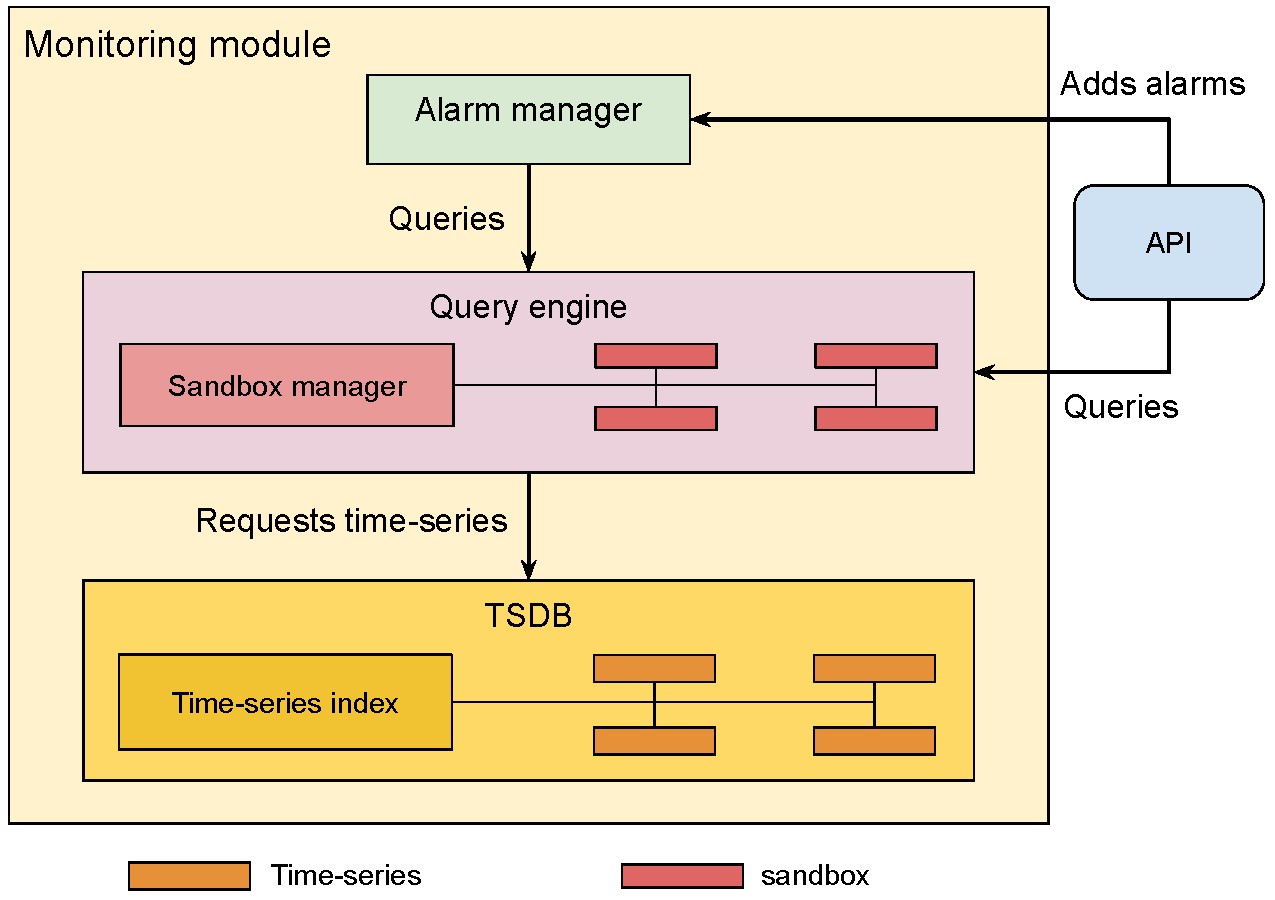
\includegraphics[width=\textwidth]{Chapters/mon_module/images/Monitoring_module.pdf}
    \caption{An overview of the monitoring module}
    \label{fig:mon_module_overview}
\end{figure}

\begin{enumerate}
    
    \item The \textbf{time-series database}, which allows the insertion and retrieval of time-series data. This time-series database makes use of an in-memory index to efficiently retrieve and insert data into the corresponding time-series.

    \item The \textbf{query engine} is the component tasked with resolving queries to the time-series database, in sum, it holds a set of sandboxes that evaluate user-provisioned queries that extract and apply aggregation functions to metrics present in the time-series database.
    
    \item Finally, the \textbf{alert manager} manages the alarms issued by the API, these alarms contain a condition that, when issued and triggered, should emit a notification to the issuing client. In sum, this component periodically verifies the issued queries using the \textbf{query engine} and propagates an event to the client whenever the condition is verified.
     
\end{enumerate}

In order to ease the explanation of these components, it is important to first describe what is the structure of the time-series data used in this framerwork, which has a similar structure to the metric types of InfluxDB \todo{cite}. 

\subsubsection{Metric  structure}

In DeMMon, a metric is composed by four elements: first, the \textbf{name}, which is a string containing the name of information that is being stored, it should be a human-readable name which is self-describing (e.g. ``CPU-USAGE''), second, the metric \textbf{tags}, that are a set of string pairs which denote attributes related to the metric that is stored, such as the hostname or cluster name of the node that emitted it, next, we have the \textbf{value}, which contains the data associated with the observed metric, and finally, we have the  \textbf{timestamp}, which contains the time at which the observation was taken. A typical example of a metric in the devised framework would be: name: ``CPU-Usage''; tags: <host:nodeX>, value: 0.3, timestamp: ``1609960731''.

It is important to mention that, in order to remain as flexible as possible, the metric values do not have a defined type. In this system, clients may use custom types (as long as they are marshallable using the JSON package provided by the golang package) \todo{cite}. This allows the devised framework to represent a multitude of different information types, such as histograms, strings, string maps, among others. For example, a decentralized service management system aimed at deploying service replicas in close proximity to the clients, may use, for example, a histogram of geographical locations, with pre-determined classes. This way, this system would have a data structure which would ease the process of finding a node in a certain geographical area.

Provided with the metric structure, we now explain how these are stored in the system. 

\subsubsection{Time-series database}

In DeMMon, time-series are sequences taken at successive equally spaced points in time, which in this system, are stored only in-memory. In this system, these sequences are indexed as a function of their name, periodicity, and tags.

In order for a certain metric (composed by: name, tags and periodicity) to be inserted into the database, a \textbf{bucket} must first be created, this is essentially a component that holds all time-series data with a certain name, periodicity and capacity. The periodicity of a bucket denotes the interval at which the sequences of points are spaced (in time), and the capacity denotes the number of points stored in each sequence, for example, a time-series with a 5-second periodicity and a capacity of 12 holds all points from the last minute. This allows the system to pre-allocate the memory necessary (using an array) for each time-series upon its creation.

Within a bucket, metrics are stored in a map and indexed by their tags, this is done by creating a key which creates the same key for each similar tag set, independent of its order: whenever a metric is inserted, its tags pairs are sorted alphabetically (by their key), and are concatenated into a single string, producing the resulting metric key. Then, using the metric key, the metric value is inserted into the corresponding time-series (a new time-series is created for that tag set if there was not one prevously in the system).

Time-series advance time in an on-demand manner, which means that any time-series, before returning values for a read or write request, verifies if its oldest value has a timestamp outside of the time-series window (as time has passed since the last check). If it has, the time series iterates its points from the oldest to the newest point, and removes all points which have exceeded its time window. It is important to mention that series concurrency is maintained using locking mechanisms, where operations which do not affect the state of the time series are executed concurrently, and operations which would otherwise change the time-series state are executed sequentially. 

\subsubsection{Query engine}

The query engine is a sub-component of the monitoring module, and it is responsible for evaluating the supplied text-based queries, transforming them into sets of instructions, and determining the final query result by executing the instructions. Keeping in mind the fact that the focus of this work is not the performance of the metric storage or querying modules and that it is still a focal point of this work to be as flexible as possible in the query language, we opted for using javascript-based interpreters to perform this work. This means that queries are essentially javascript code, meaning that users have infinite control on the behavior of their queries, provided these dont exceed the query timeout.

In order to provide this functionality we opted for using the package Otto \todo{insert citation}, this package provides access to javascript ``virtual machines'' that essentially take a string containing a javascript script, and build an AST from the parsed code, then this AST is executed and the result is returned by the VM, which allows a practically infinite range of query options. In order to allow users to access the time-series stored in the TSDB without directly doing so (as the user-defined queries could potentially alter internal state of time time-series), the query engine provides every Otto virtual machine access to the following functions, which return time-series from the database:

\begin{enumerate}

    \item SelectLast(Bucket\_Name, <Tag\_set\_regex>), this function returns the last point for every time-series which are in the supplied bucket that match the provided tag set regex. The way the tag set regex matching works is: for every time series present in the specified bucket, if all of the tag keys in the supplied regex match all of the time series tags, then the time series is returned. An example of the usage of this function woud be, for example: ``selectLast(CPU\_USAGE, <host:.*, cluster:cluster1>)''
    
    \item Select(Bucket\_Name, <Tag\_set\_regex) this function behaves similarly to selectLast, however it returns all points in all matched time series.
    
    \item SelectRange(Bucket\_Name, <Tag\_set\_regex>, startDate, endDate), this function behaves similarly to select and selectLast, however its arguments take an additional time range, and instead of only returning the last value it returns all points inside the supplied range.
    
\end{enumerate}

With these 3 functions, clients can select either a partial set of points or the totality of points from every time series stored in the system, these time series are then usable in the javascript code.  

We believe covers the most common use cases for metric selection. These metrics, upon selection, can then be aggregated in any way the user specifies in the query (since they are composed of user-defined code). In order to ease the design of queries and prevent developers from rewriting the same aggregation functions, the query engine also provides some aggregation primitives which can be applied to one or more timeseries such as: Max, Min and Average.

After the selection and aggregation of metrics, the resulting values are returned by placing them in a variable denoted ``result'' (this can be omitted if the query simply returns a set of values). Any query executed in deMMon can only result in one of two options: a single time series or an array of time series. Given this, in order to allow the creation of new time series during the query process, there are two additional functions available to the virtual machines: the first is called ``NewTimeSeries'', which creates a new time series, this function takes as argumments the name, tags and values which will integrate the time series; second, we have the function called ``NewObservable'' which takes the observed value and a timestamp and  to create a new metric point which can be added to time series.

 With this, we now provide some examples of possible queries along with a brief description of what they do:

\begin{enumerate}
    \item ``Avg(SelectLast(CPU\_USAGE, <host:.*, cluster:cluster1>))'' this query selects the metrics with the name ``CPU\_USAGE'' for all hosts which belong to cluster with name ``cluster1'' and returns the average of all the points.
    
    \item ``SelectLast(Nr\_services, <tenant:tenant10>, startDate, endDate)'' this query returns the timeseries for the metric called ``Nr\_services'' for the tenant with name ``tentant10'' during the provided time range.

    \item ``SelectLast(Nr\_replicas, <tenant:tenant10,service:service10>)'' this query returns the timeseries for the metric called ``Nr\_replicas'' for the tenant with name ``tentant10'' and service named ``service10'' during the provided time range.
    
    \item \todo{meter mais um exemplo de uma query custom}
    
\end{enumerate}

With this, clients are able to, through the API, obtain and manipulate data from the time series database using text-based queries. Furthermore, as the type of the value of each metric is not enforced, clients may store their metrics in custom data structures tailored for their use-cases.

\subsubsection{Alarm manager}

The alert manager is the last component of the monitoring module, it is responsible for managing the alarms issued to the monitoring module. Alarms are essentially sets of parameters which contain, among others, a condition to observe (e.g. the percentage of CPU usage). This component is essentially responsible for periodically verifying this condition and issuing notifications to the client whenever the condition is observed. Alarms are paramount to prevent applications from having to periodically access the API to verify the condition themselves, effectively saving bandwidth.

In deMMon, an alarm is composed by the following components: 

\begin{enumerate}
    \item \textbf{Query} - This denotes the query to perform periodically, this query must return a boolean value.
    
    \item \textbf{Periodicity} - The periodicity denotes how often the query is evaluated, and how often notifications are sent to the client that issued the alarm
    
    \item \textbf{Backoff time} - The backoff time is a duration decreases the rate at which the monitoring module emits notifications, which would otherwise happen at the alarm periodicity every time the alarm is verified (e.g. if the alarm periodicity is low).
    
    \item The \textbf{watch list} is a set which, for every item, contains both a name and a set of tag filters. Whenever the alarm manager receivers an alarm containing a watchList, in addition to performing the verification at the specified periodicity, it also performs the verification whenever any time series matching the watch list is changed. The rates at which the alarm is verified in this manner also respects the backoff time.
    
    \item The \textbf{CheckPeriodic} is a boolean variable denoting if the alarm should be verified periodically. When false, the alarm manager does not check the metrics at every \textbf{Periodicity} seconds, effectively saving CPU time. This option is meant to be used together with the watch list, for example, for checking a parameter which is rarely altered. It is important to mention that if this parameter is set to false, then time-based effects such as the expiration of either time series or points are not observed (as the alarm is not checked periodically).
\end{enumerate}

The monitoring module, whenever it receives a new alarm, essentially adds it to a priority queue containing all the alarms which uses the time of reception of the alarms plus their periodicity as their key to the queue. Using this data structure, alarms are sorted by the time at which they need to be verified. Then, the monitoring module continuosly obtains and removes the first item of the queue, containing the next alarm to verify out of all issued alarms. After this, monitoring module waits until it is time of verification of that alarm (i.e. the time of reception of the alarm plus its periodicity), then verifies it, and adds it to the queue with a new timestamp corresponding to the current time plus the alarms' periodicity.

Whenever the alarm is verified and the result of its query returns ``true'', the alarm manager verifies if it has emitted a notification for that alarm in the last ``Backoff time'', and issues a notification to the client if it hasn't.

